\documentclass[titlepage]{article}
\usepackage[ukrainian]{babel}
\usepackage{listings}
\usepackage{amsmath}
\usepackage{fontspec}
\setmainfont{Times New Roman}
\usepackage{setspace}
%\spacing{1.7}
\usepackage{fancyhdr}
\usepackage{titling}
\usepackage[a4paper, top = 20mm, bottom = 20mm, left = 25mm, right = 15mm]{geometry}
\usepackage{graphics}

\lstset{
	basicstyle=\large,
	breaklines = true,
	language = matlab,
	breakatwhitespace = true,
	numbers = left,
	numberstyle = \tiny,
	columns = flexible,
	frame=tb,
	tabsize=4
}

\makeatletter
\renewcommand\normalsize{%
\@setfontsize\normalsize{14pt}{15pt}}
\makeatother

\newcommand\makelisting[1]{\lstinputlisting[title=#1]{../#1} \vspace{1cm}}

\preauthor{\begin{flushright}}
\postauthor{\end{flushright}}

\fancypagestyle{empty}{%
	\renewcommand{\headrulewidth}{0pt}
	\cfoot{\normalsize2016}
	\chead{\uppercase{київський національний університет імені тараса шевченка}}
}

\begin{document}

\title{\normalsize Лабораторна робота учбової практики}
\author{\vspace{5cm}Виконав: \protect\\ студент 4-го курсу \protect\\ спеціальність математика \protect\\ Шатохін Михайло}
\date{}
\maketitle
\section{Постановка задачі}
Необхідно побудувати інтерполяційний сплайн $S(x, u)$ другого степеня дефекту 1, з крайовими умовами типу II.
\section{Код}
Функція, що здійснює перевірку правильності побудови сплайну: побудову графіків та розрахунок сіткової норми.
\makelisting{main.m}
Функція, що здійснює побудову сплайна.
\makelisting{CreateSpline.m}
Побудова матриці за допомогою других похідних $M_i$.
\makelisting{CreateSEMatrix.m}
Розв'язання системи лінійних рівнянь за допомогою методу квадратного кореня.
\makelisting{SolveSE.m}
Формування коефіцієнтів сплайну.
\makelisting{FormSpline.m}
Нижче наведений результат роботи програми:
\begin{figure}[h]
\hspace{-3cm}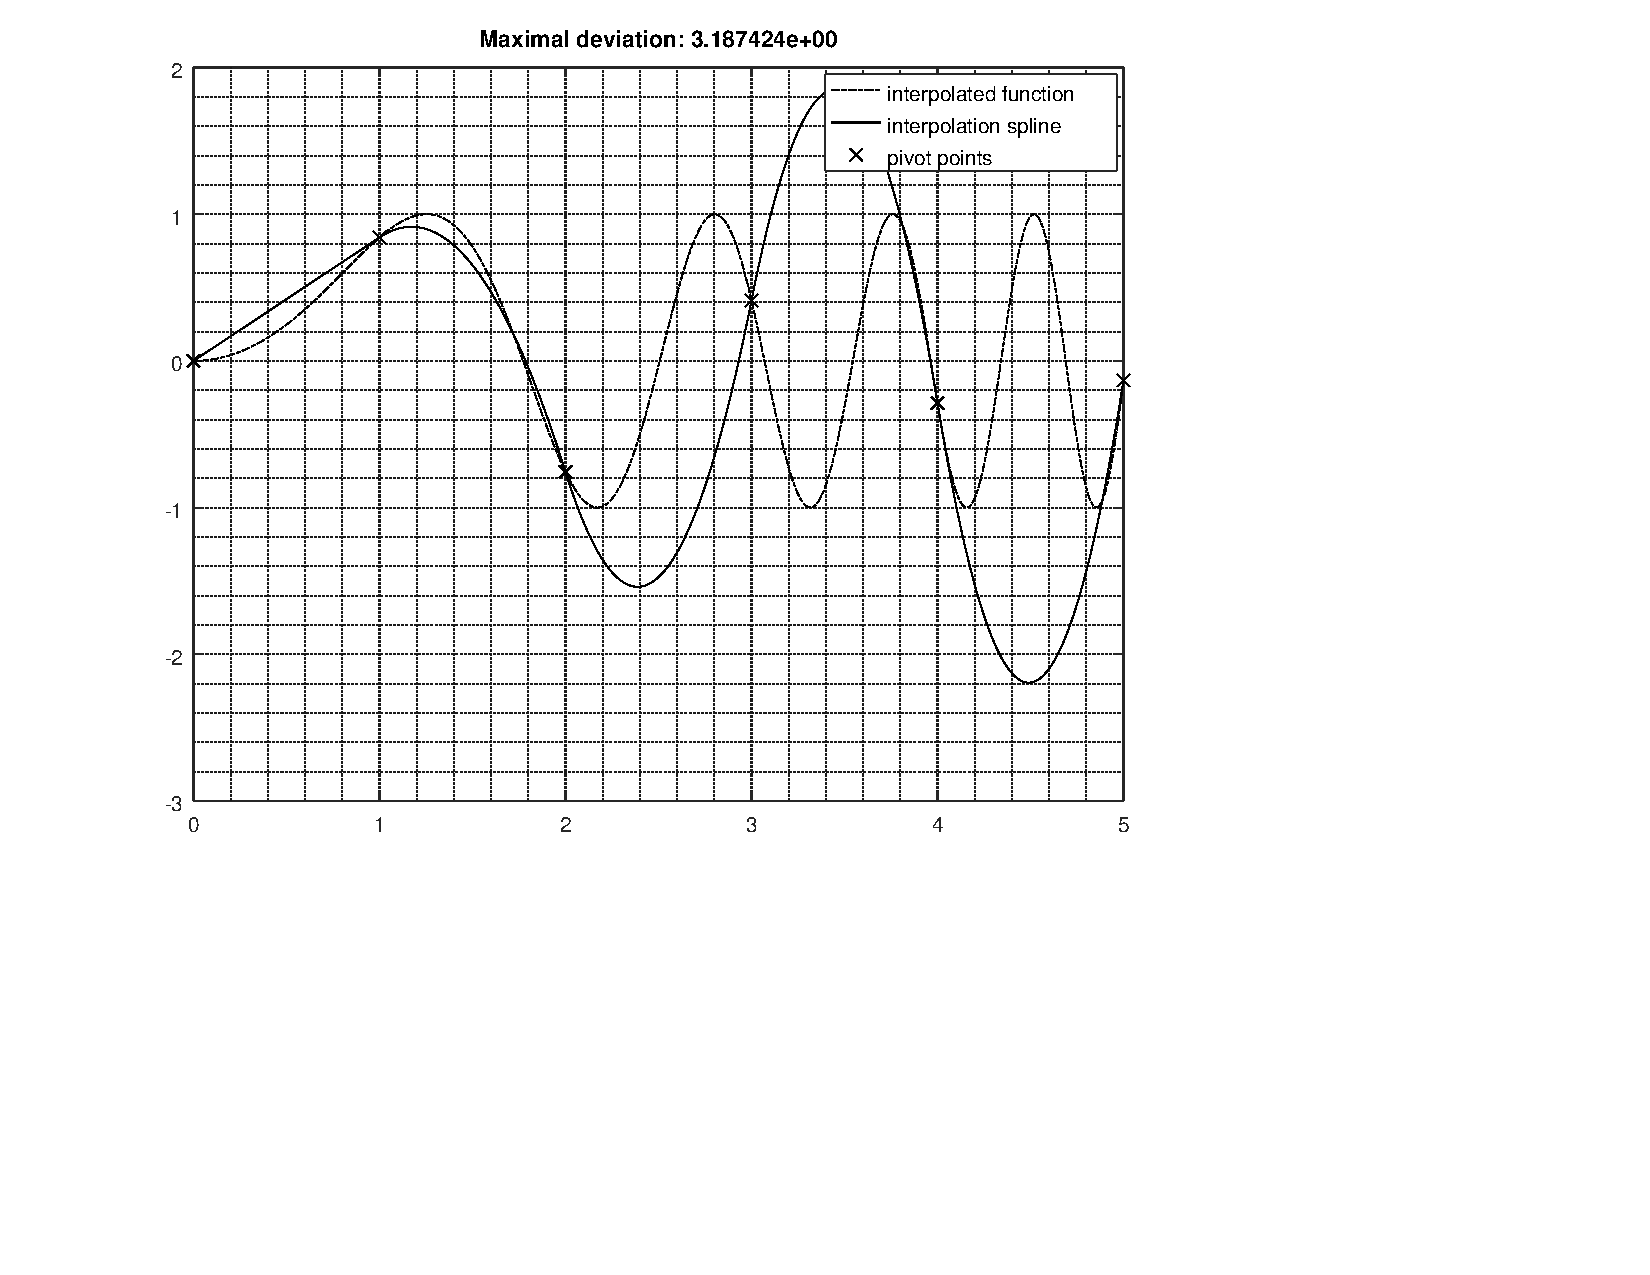
\includegraphics[page=1]{../result.pdf}
\end{figure}
\begin{figure}[h]
\hspace{-3cm}\includegraphics[page=2]{../result.pdf}
\end{figure}
\end{document}